% This is LLNCS.DOC the documentation file of
% the LaTeX2e class from Springer-Verlag
% for Lecture Notes in Computer Science, version 2.4
\documentclass{llncs}
\usepackage{llncsdoc}
\usepackage[utf8]{inputenc}
%
\begin{document}

\title{Cyber-insurance \& endogenous network formation}

\author{Håvard Råmundal Halse\inst{1}, Jonas Hoemsnes\inst{1} \and Gergely Biczók\inst{2}}

\institute{Dept. of Telematics \\
Norwegian University of Science and Technology \\ \{havahals, jonashoe\}@stud.ntnu.no
\and
Dept. of Telematics \\
Norwegian University of Science and Technology \\ gbiczok@item.ntnu.no}

\maketitle
%

\begin{abstract}
Cyber-insurance is a powerful economic concept that can help companies in the fight against cybercrime. From the early 80s, several researchers claimed that cyber-insurance had a bright future, were it would become a huge economical tool for handling residual cyber-risks.

However, both the European and US cyber-insurance market have failed to grasp its promising potential. To fully grasp this potential they need  innovative approaches to handle the unique problems of cyber-insurance.

This paper find and characterize network structures with properties that make them superior as cyber-insurance. And creates several models for forming these network structures. In every model, new properties that relate the model to the real-world and real-world insurance products are added. The results show that insurers can use the insurance premium as a tool for determining the resulting formation of the network, and if set to the right level, these superior structures will evolve. 

We believe our findings could help the cyber-insurance market evolve, by giving the insurers a proper tool to better analyze and control formation of cyber-insurance networks. 

\end{abstract}
%
\section{Introduction to cyber-insurance}
Security breaches are increasingly prevalent in the Internet age causing huge financial losses
for companies and their users. When facing security breaches and risk, there are typically four ways to act \cite{bolot:cyber}:
1. Avoid the risk, 2. Retain the risk, 3. Self protect and mitigate the risk and 4. Transfer the risk.

%\begin{enumerate}
%\item Avoid the risk
%\item Retain the risk
%\item Self protect and mitigate the risk
%\item Transfer the risk
%\end{enumerate}
The ICT industry have so far tried to prevent risks with a mixture of options two and three. This has lead to many different techniques and software trying to detect threats and anomalies, to protect the users and infrastructure. Firewalls, intrusion- detection and prevention systems, are some of the solutions. These will reduce the risk, but do not eliminate the risk completely. Although they are all good and needed actions, it is impossible to achieve perfect cyber-security, due to many reasons: Threats are continuously evolving, there will always be accidents and security flaws, attackers have different intentions, network externalities and free-riding in security networks, the lemons-market in security products, misaligned incentives between users and product vendors, and many more. 
This is why we need cyber-insurance, as an fourth option, to handle the residual risk \cite{bolot:cyber2,ranjan:cyber}.

The market for cyber-insurance emerged in the late 80's, when security software companies began collaborating with insurance companies to offer insurance policies together with their security products. From a marketing perspective, adding insurance helped highlighting the supposedly high quality of the security software. Nevertheless, this new product was a comprehensive solution, which dealt with both risk reduction and residual risk \cite{bolot:new}. Continuing into the beginning of the new millennium, several companies started offering standalone cyber-insurance, which sat the frame for the current insurance product. However, as found in the papers \cite{ccost,evolvingcyber,CFCunder} both the US and the european market have not managed to reach its promising potential. Companies are weekly suffering from successful attacks, but most firms still have not acquired cyber-insurance. 
Researchers claim that the main reasons that cyber-insurance is struggling is the three unique problems, information asymmetry, correlated risk and interdependent agents \cite{bohme2010modeling}. 
\paragraph{Information asymmetry.}
Information asymmetry arises when one side of a transaction or decision has more or better information than the other party. There are two different cases of information asymmetry. The first one is called adverse selection, where one party simply has less information regarding the performance of the transaction. A good example for the cyber-industry, where an insurer has trouble confirming whether your computer/network is "healthy".
The other information asymmetry scenario is called moral hazard. It occurs after the signing of the contract, where one party deliberately takes some action that makes the possibility of loss higher, e.g. choosing not to lock your door. 
      
\paragraph{Correlated risk.}

Another big concern regarding cyber-insurance, is the correlated risk. Among other things, the problem occurs due to the need for standards. Standardization is an important part of the business of computers and computer networks. Generally it enables computers to communicate, install and use different software. A good example is operative systems for personal computers, today we only have a small set of operative systems available, and these systems are standardized, so they can use the same communication channels. The standards generate a lot of the value in the ICT industry, but they also make many threats possible. All systems that use the same standards, create a large number of similar exposure units which could be exploited at the same time. 
Thus create a significant difficulty for the cyber-insurance industry, because when a security breach occurs there is a high probability that it will occur to a large number of people.
 
 \paragraph{Interdependent security.}
Another problem in the ICT industry is interdependent security, meaning that you are not only dependent on your own investment in security, but also on everyone else's. 
Investment in security generates positive externalities, and as public goods, this encourages free riding. The problem is that the reward for a user investing in self-protection depends on the security in the rest of the network. i.e. The expected loss due to a security breach at one agent in the network, is not only dependent on this agent's level of investment in security, but also on the security investment done by adjacent agents, and their adjacent agents and so forth.
  
The cyber-insurance market seem to have a huge potential, but needs some new thinking to fully take advantage of it. We will take a new approach where we focus on finding network structures that will be beneficial for cyber-insurance, and see if it i possible for insurers to force these structures to evolve.


\section{Fixed-Period Problems: The Sublinear Case}
%
With this chapter, the preliminaries are over, and we begin the search
for periodic solutions \dots
%
\subsection{Autonomous Systems}
%
In this section we will consider the case when the Hamiltonian
$H(x)$ \dots
%

\section{Modeling Cyber-insurance}
\section{Models}
There are many examples of nodes that need to establish connections with eachother.
For example, when a firm is outsourcing tasks, cooperating or depending on other
firms in some way. Such scenarios could be modeled, as networks where the nodes
represents the firms and the links between them are their dependencies. However,
the link between nodes involves some risks, such as: will the company deliver at the
reported time, to the reported costs, what happens if it fails to deliver, what if the
company goes bankrupt etc. To handle these risks, we need cyber-insurance.

From the insurer’s point of view, a problem with cyber-insurance is to define and calculate risk, because the network structure is
undefined. If an insurer were able to predict the network structure, the calculations
of overall risk would be realizable. The situation could be even better if the insurer
could force the structures found earlier to evolve, hence, ensuring a higher
total payoff for the network. In summary, star topologies, or
star-like topologies, have a fixation probability that exceeds the fixation probability
of circulation graphs. Star structures also have a desirable property of minimizing the
average path length, i.e. minimizing the cost spent on establishing links. Finally, the
clique has a nice property of being able to achieve super-critical payoff, as showed in
[Blu11]--fix. Both the clique and star have the possibility of amplifying or suppressing selection and drift. This is favorable, because if the insurer is able to ensure that the nodes have a certain security level, one can prevent viruses from spreading.

In our models a node is an agent who is either insured or not, and the nodes’ goal is to maximize its payoff, by establishing links with other nodes. Our goal for the models is to find out if and how an insurer can force these cyber-insurance networks to evolve into the desirable structures mentioned in previous sections.
The different parameters used to model the formation games are denoted as follows: The insurance premium is $I_{l}$, the expected risk cost is represented by $r$. $\beta$ represents the benefit of establishing a link. When establishing a link, the decision is a bidirectional decision.  
 
\section{Model 1: Including maximum node degree and bonus}
In real world networks, such as in the manufacturing industry, software development firms and many other types of business, in some scenarios a product can usually not be completed without outsourcing some of the work needed. For the manufacturer, it could be beneficial to buy certain parts from others instead of producing them on his own. A software product might need the combined knowledge from different firms. Thus the firm that outsources tasks is dependent on the other firms, and will not reach its goal before the other firms deliver their contribution. When the product is finished the company gets paid.
To model this scenario we introduce a maximum node degree, $m$, per node, which represents the number of partners needed to complete a task. Additionally a bonus $\gamma$ represents the payoff a node receives when $m$ links are established. 

When establishing a link between two insured nodes, the payoff the nodes will receive is as described in Eq.(\ref{eq:itoi}).
Let $U_{i}$ denote the payoff of a node with degree i, and let $U_{i+1}$ be the payoff
a node will receive if it establishes a new link.
\begin{equation}
    U_{i+1}= 
\begin{cases}
    \beta - I_{l},& \text{if } i = 0\\
    U_{i}+\beta -I_{l},& \text{if }  i>0\\
    U_{i}+\beta -I_{l}+\gamma,& \text{if } i=m-1
    
\end{cases}
\label{eq:itoi}
\end{equation}

\subsection{Analysis}

For nodes to connect to each other, the change in payoff has to be positive: $U_{i+1} > U_{i}$. However, we also need to consider the bonus received when reaching the maximum node degree, $m$. 
To model this, we add the possible bonus divided on the number of links required to reach the bonus($\frac{\gamma}{m-i}$) in the decision process every time a node is considering to establish a link. 
In this way, nodes with higher degree will be more risk willing than nodes with low degree. For example, an insured node is more likely to accept a risky link when it only needs one more link to reach the goal, compared to when it need several more links to reach the goal.

We start our analysis by analyzing the four possible link establishment scenarios, insured
to insured, insured to non-insured, non-insured to insured, and non-insured to noninsured.
When establishing a link between two insured nodes, the payoff the nodes will receive is as described in Eq.(\ref{eq:itoi}).
\begin{equation}
    U_{i+1}= 
\begin{cases}
    \beta - I_{l},& \text{if } i = 0\\
    U_{i}+\beta -I_{l},& \text{if }  i>0\\
    U_{i}+\beta -I_{l}+\gamma,& \text{if } i=m-1
    
\end{cases}
\label{eq:itoi}
\end{equation}
As described earlier we need to include the possibility of reaching the goal in the decision, and thus for insured nodes to connect to each other, Eq.(\ref{eq:itoi2}) has to hold.
\begin{eqnarray}
U_{i}+\beta-I_{l}+\frac{\gamma}{m-i}&>U_{i} \nonumber \\ 
\beta-I_{l}+\frac{\gamma}{m-i}&>0 \nonumber \\ 
\llap{$\rightarrow$\hspace{50pt}} \beta+\frac{\gamma}{m-i}&>I_{l} 
\label{eq:itoi2}
\end{eqnarray}

The payoff an insured node receives when connecting to a non-insured node is as follows:
\begin{equation}
    U_{i+1}= 
\begin{cases}
    \beta  - I_{l} -r,& \text{if } i = 0\\
    U_{i}+\beta -I_{l}-r,& \text{if }  i>0\\
    U_{i}+\beta -I_{l}-r+\gamma,& \text{if } i=m-1
\end{cases}
\label{eq:itonoti}
\end{equation}
To establish a connection from an insured node to a non-insured one, the following has to hold:
\begin{eqnarray}
U_{i}+\beta-I_{l}-r+\frac{\gamma}{m-i}&>U_{i} \nonumber \\ 
\beta-I_{l}-r+\frac{\gamma}{m-i}&>0 \nonumber \\ 
\llap{$\rightarrow$\hspace{50pt}} \beta+\frac{\gamma}{m-i}-r&>I_{l} 
\end{eqnarray}

When a non-insured node connects to another non-insured node, this is the payoff they both will receive:
\begin{equation}
    U_{i+1}= 
\begin{cases}
     \beta -r,& \text{if } i = 0\\
    U_{i}+\beta -r,& \text{if }  i>0\\
    U_{i}+\beta -r +\gamma,& \text{if } i=m-1
\end{cases}
\label{eq:noitonoti}
\end{equation}
To establish the connection, the following equation has to hold:
\begin{eqnarray}
U_{i}+\beta-r+\frac{\gamma}{m-i}&>U_{i} \nonumber \\ 
\beta-r+\frac{\gamma}{m-i}&>0 \nonumber \\ 
\llap{$\rightarrow$\hspace{50pt}} \beta+\frac{\gamma}{m-i}&>r
\end{eqnarray}
In the case of a non-insured node wanting to establish a link with an insured node, the payoff is a strictly increasing function, see Eq.(\ref{eq:noitoti}), and thus a non-insured node will always connect to an insured node if possible.
\begin{equation}
    U_{i+1}= 
\begin{cases}
    \beta,& \text{if } i = 0\\
    U_{i}+\beta,& \text{if }  i>0\\
    U_{i}+\beta +\gamma,& \text{if } i=m-1
\end{cases}
\label{eq:noitoti}
\end{equation}

\subsection{Result and findings}

If we want a clique of only insured nodes, we have to ensure that insured nodes connect to each other, and that they do not establish connections to non-insured nodes.
We know that an insured node would want to connect to another insured node if  Eq.(\ref{eq:itoi2}) is satisfied. 
In the equation we see that the expected bonus per established link is increasing. Thus, if an insured node of degree zero is willing to connect to another insured node, then every insured node with a degree higher than zero would also like to connect to another insured node. To ensure that insured nodes connect to eachother this equation has to hold:
\begin{equation}
\beta+\frac{\gamma}{m}>I_{l}
\label{eq:conditionitoi}
\end{equation}
We also want to ensure that insured nodes never establish links with non-insured nodes, from Eq.\ref{eq:itonoti} we see that this has to hold:
\begin{equation}
\beta+\frac{\gamma}{m-i}-r < I_{l}
\label{eq:conditionitonoti}
\end{equation}
This can be simplified, if one can ensure that the most risk willing insured node, i.e. the node with degree $m-1$, does not establish links with non-insured nodes. Then we know that no insured node with degree less than $m-1$ will establish links with non-insured nodes. From this we get equation Eq.(\ref{eq:condition-i-to-noti}).

\begin{eqnarray}
\beta+\frac{\gamma}{m-(m-1)}-r&<I_{l} \nonumber\\
\llap{$\rightarrow$\hspace{50pt}} \beta+\gamma-r&<I_{l}
\label{eq:condition-i-to-noti}
\end{eqnarray}

To summarize, Eq.(\ref{eq:conditionitoi}) and Eq.(\ref{eq:condition-i-to-noti}) give the final limitation on the link insurance cost, Eq.(\ref{eq:final-insurance-clique-condition}). If this equation is satisfied, the resulting network will contain a clique of only insured nodes.
\begin{equation}
\beta+\gamma-r<I_{l}<\beta+\frac{\gamma}{m}
\label{eq:final-insurance-clique-condition}
\end{equation}
For this to even be possible, $\beta+\gamma-r<\beta+\frac{\gamma}{m}$, i.e. Eq.(\ref{eq:noinsuredcliqueconditon}) has to hold. This equation reflects that as the risk to bonus ratio gets smaller, it gets more and more difficult to ensure a clique of only insured nodes. 
\begin{eqnarray}
\gamma-r &<\frac{\gamma}{m}\nonumber \\
1-\frac{r}{\gamma}&<\frac{1}{m} \nonumber \\
\llap{$\rightarrow$\hspace{50pt}}1-\frac{1}{m}&<\frac{r}{\gamma}
\label{eq:noinsuredcliqueconditon}
\end{eqnarray}

It is also useful to know when non-insured nodes connect to each other. This happens when Eq.(\ref{eq:noitonoti}) is satisfied. This equation is dependent on the node degree, and thus for the first link to be established from a non-insured node, the expected payoff has to be higher than the risk($\beta+\frac{\gamma}{m}>r$). If the risk is too high, then the non-insured node must establish links with insured nodes before it could be willing to establish risky links.

With these findings, an insurer can determine the outcome of the network formation game by adjusting the insurance cost parameter.
If he wants a clique of only insured nodes Eq.(\ref{eq:final-insurance-clique-condition}) has to
hold. However, it is easy to relax the condition, so that insured nodes only connect to, $j=1,2,3..m$ non-insured nodes.
   This is done by changing Eq.(\ref{eq:condition-i-to-noti}) to $\beta+\frac{\gamma}{m-(m-j)}-r<I_{l}$, which
    gives us Eq.(\ref{eq:lower-boundary-link-insurance-cost}).

\begin{equation} 
\beta+\frac{\gamma}{j}-r<I_{l}
\label{eq:lower-boundary-link-insurance-cost}
\end{equation} 

\subsection{Simulation of the results}
For the first simulation the parameters are set to the following: $\beta=0.9, I_{l}=0.7, r=0.5, \gamma=0.2 \text{ and }m=4$, in order to satisfy condition Eq.(\ref{eq:final-insurance-clique-condition}), and enable all nodes to reach their maximum degree.  

\begin{figure}[h]
\centering
  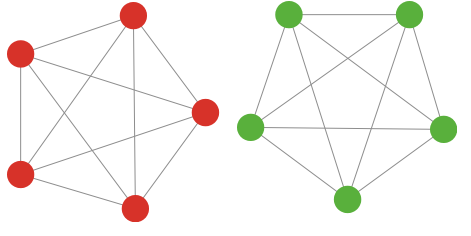
\includegraphics[scale=0.5]{../Figures/BonusGameInsuredClique.png}
  \caption{\label{fig:bonusoptimal} Two cliques, one consisting of insured agents the other consists of non-insured. All nodes have reached their goal. }
\end{figure}
As we see in Figure \ref{fig:bonusoptimal}, the results were as expected, the cost of insuring a link satisfied the conditions found earlier, and thus the result was two cliques, one consisting of only insured nodes and the other of non-insured nodes.
The price of anarchy in this scenario is 1, i.e. the socially optimal outcome. 

In the second simulation we set the parameter $m=5$, and kept the other variables unchanged. The resulting network was as expected the same as in the last simulation, but since the nodes did not reach their maximum degree, the price of anarchy is less than one. The price of anarchy can be seen in Eq.(\ref{eq:model-bonus-poa}).
\begin{eqnarray}
PoA&=\frac{\text{Sum of payoffs}}{\text{Sum of Socially optimal payoffs}}  \nonumber \\
PoA&=\frac{5\times 4\times (0.9-0.7)+5\times 4\times(0.9-0.5)}{5\times 4\times (0.9-0.7)+5\times 4\times(0.9-0.5)+5\times (2\times 0.9-0.7-0.5 + 2 \times 0.2)}\nonumber \\
PoA&=\frac{12}{17}
\label{eq:model-bonus-poa}
\end{eqnarray}

When we changed the link insurance cost to $I_{l}=0.5$, the resulting networks change. Now we found that the insured nodes are willing to establish risky links to reach their maximum degree. Some of the resulting networks can be seen in the figures \ref{fig:bonusvolating:a} and \ref{fig:bonusvolating:b}. In figure \ref{fig:bonusvolating:a} the price of anarchy is $0.95$, and in figure \ref{fig:bonusvolating:b} the price of anarchy is $1$, i.e. it has reached the socially optimal outcome.


\begin{figure}
  \centering
  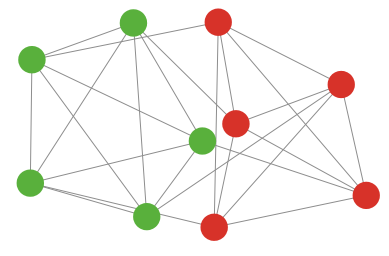
\includegraphics[scale=0.5]{../Figures/BonusGameViolatingOptimal.png}
  \caption{\label{fig:bonusvolating:b}Every non-insured node is connected to one insured node, this is the optimal outcome with these parameters.}
\end{figure}
  
\section{Model 2: Including bulk insurance discount}

 It seems to be common for insurance companies to offer discount to their customers if the customers choose to combine some or all of their insurances with them. We would like to introduce a discount rate dependent on the degree of the node. In a real-world scenario where nodes have an option of acquiring insurance or not, this will make it more attractive for nodes with high degree to acquire insurance, and the discount could act as an incentive for nodes to also acquire insurance. 

How insurance companies choose to formulate their discount rate might vary. One solution might be to follow a strict 5$\%$ discount per new connection, or let the discount follow a power law, or a log-function etc. We choose to follow a discount rule which directly reflects the node's degree.

\subsection{Analysis}
The price for adding a new link follows the equation:
\begin{equation}
\frac{I_{l}}{i+1}
\label{eq:discount0}
\end{equation}
Here, $i$ is the node's current degree. This means that the more links a node establishes the cheaper the link insurance will be. 

\subsubsection{Discount and Bonus model}

When the discount is applied to model 1, the only connection scenarios that is worth considering in this model is the ones where insured nodes connects to other insured nodes or when insured nodes connects to non-insured nodes.

When insured nodes are considering to establish links with eachother, their payoff functions are as shown in Eq.(\ref{eq:discount1}).  
\begin{equation}
    U_{i+1}= 
\begin{cases}
    \beta - I_{l},& \text{if } i = 0\\
    U_{i}+\beta -\frac{I_{l}}{i+1},& \text{if }  i>0\\
    U_{i}+\beta -\frac{I_{l}}{i+1}+\gamma,& \text{if } i=m-1
\end{cases}
\label{eq:discount1}
\end{equation}
For insured nodes to connect to eachother Eq.(\ref{eq:model4-bonus-i-to-i}) has to hold.

\begin{eqnarray}
U_{i}+\beta-\frac{I_{l}}{i+1}+\frac{\gamma}{m-i}&>U_{i} \nonumber \\ 
\beta-\frac{I_{l}}{i+1}+\frac{\gamma}{m-i}&>0 \nonumber \\ 
\llap{$\rightarrow$\hspace{50pt}}\beta +\frac{\gamma}{m-i}&>\frac{I_{l}}{i+1}
\label{eq:model4-bonus-i-to-i}
\end{eqnarray}

When insured nodes are considering to connect to non-insured nodes, their payoff functions are as shown in Eq. (\ref{eq:model4-bonus-i-to-ni}).
\begin{equation}
U_{i+1}= 
\begin{cases}
    \beta - I_{l}-r,& \text{if } i = 0\\
    U_{i}+\beta -\frac{I_{l}}{i+1}-r,& \text{if }  i>0\\
    U_{i}+\beta -\frac{I_{l}}{i+1}-r+\gamma,& \text{if } i=m-1
\end{cases}
\label{eq:model4-bonus-i-to-ni}
\end{equation}
For this to happen Eq.(\ref{eq:model4-bonus-i-to-ni-final}) has to hold.

\begin{eqnarray}
U_{i}+\beta-\frac{I_{l}}{i+1}+\frac{\gamma}{m-i}-r&>U_{i} \nonumber \\ 
\llap{$\rightarrow$\hspace{50pt}}\beta+\frac{\gamma}{m-i}&>r+\frac{I_{l}}{i+1}
\label{eq:model4-bonus-i-to-ni-final}
\end{eqnarray}

\subsection{Result and findings}

We want to find the condition for separating insured and non-insured nodes. The first step is to guarantee that insured nodes connect to eachother. To ensure that this happens, we need to find the condition for the lowest expected increase in payoff, i.e. at node degree zero. If nodes are willing to establish links at this point, then they will also be willing at all degrees higher than zero.
At degree zero there is no discount on the insurance link cost, and thus if Eq.(\ref{eq:conditionitoi}) from model 1 holds, insured nodes will connect to other insured nodes.

The condition for guaranteeing that insured nodes do not connect to non-insured nodes has changed, we know that if an insured node does not want to establish a link with a non-insured node at degree $m-1$, then neither will any insured node with degree lower than $m-1$ do so. From this we find the condition in Eq.(\ref{eq:model4-bonus-i-not-ni})
\begin{eqnarray}
U_{i}+\beta-\frac{I_{l}}{m}+\frac{\gamma}{m-(m-1)}-r&<U_{i} \nonumber \\ 
\beta+\gamma-r&<\frac{I_{l}}{m}\nonumber \\ 
\llap{$\rightarrow$\hspace{50pt}}m(\beta +\gamma-r)&<I_{l}\nonumber
\label{eq:model4-bonus-i-not-ni}
\end{eqnarray}
This is a very strong condition, because the only way this can happen is if $\beta+\gamma-r<\frac{1}{m}$.  This shows us that when the incentives for establishing links increase, it gets more and more difficult for the insurer to guarantee a clique of only insured nodes. 
The final condition for ensuring a clique of only insured nodes is shown in Eq.(\ref{eq:model4-final-condition-insured-clique}).

\begin{equation}
m(\beta +\gamma-r)<I_{l}<\beta+\frac{\gamma}{m}
\label{eq:model4-final-condition-insured-clique}
\end{equation}

The quantum discount results in an overall higher payoff for the insured nodes, since the cost of insuring a new link becomes cheaper. This means that the insured nodes will have a higher incentive to create links, making it harder for the insurer to separate insured and non-insured nodes.

We see that the problem of separating the two node types have increased compared to the previous model, meaning that if we have a network where the insurer has managed to separate them, the price of anarchy is also higher compared to a similar scenario in the first model. 

\section{Model 3: Network externalities}
In the earlier models when a node established a connection the change in utility were only dependent on fixed variables, and not dependent on the rest of the network. In many real world scenarios it is more realistic that a node will be strongly affected by the indirect connections to other nodes. Social relationships between nodes are good examples of such networks, where each person offer benefits in terms of favors, information etc. 

We apply the results from the paper from Jackson and Wolinsky \cite{jackson1996strategic} and use a network formation game found in \cite{jackson2005survey} to study indirect network effects in our model. 

The benefits a player receives in this game are calculated as follows: In addition to the benefit from the direct connection, a node will also benefit from "friends of the friend", and "friends of the friends of the friend" etc. This is achieved by letting the payoff be calculated relative to the distance between the nodes. $\beta$ now depends on the minimum number of hops to the node. We want the benefit to decrease with distance, therefore we need the limitation: $0<\beta<1$. 
The total payoff for a node is:

\begin{equation}
\sum_{j\neq i}^{} \beta_{ij}^{d(ij)} - \sum_{j:ij\in g}^{} {c}_{ij}, 
\label{eq:connecetionGame}
\end{equation}

Where $d(ij)$ represents the shortest path between node $i $ and node $j $, and ${c}_{ij}$ represents node i's cost of establishing a link between the two nodes. 

In the paper \cite{jackson1996strategic}, the authors analyze the networks created with these rules with two different approaches, one with focus on efficiency and the other on stability.  The optimal network is of course both efficient and stable, but as we shall see there are some conflicts between efficiency and stability. Matthew, et.al. showed that an efficient network is:
\begin{enumerate}
\item \textit{a complete graph $g^N$ if $c<\beta - \beta^2$,}
\item \textit{a star encompassing every node if $\beta - \beta^2 < c < \beta + \frac{(N-2)}{2}\beta^2$,}
\item \textit{an empty network (no links) if $\beta + \frac{(N-2)}{2}\beta^2 < c$.}
\end{enumerate}

The most efficient structure is a star structure which encompasses every node. A star structure has the characteristics of minimizing the average path length and uses the minimum number of links ($N-1$) required for including every node. However, it is not preferable to be the center node, due to the cost of all the direct links. 
This structure provides the highest overall payoff for the network, but this network is not necessarily stable.

When analyzing the stability of the network, by using the definition of pairwise stability, Jackson and Wolinsky found four different stability conditions:

\begin{enumerate}
\item \textit{a pairwise stable network consists of at most one (non-empty) component,}
\item \textit{if $c<\beta - \beta^2$, the unique pairwise stable network will be a complete graph $g^N$, }
\item \textit{if $\beta - \beta^2 <c < \beta $, a star encompassing every node will be pairwise stable, although not necessarily the unique pairwise stable graph,}
\item \textit{if $\beta < c$, any pairwise stable network which is nonempty is such that each player has at least two links and is thus inefficient. }
\end{enumerate}
We see that stability condition 2 is the same as efficiency condition 1, and therefore if this condition is fulfilled, the network is both stable and efficient. 
Condition 3 shows us why the efficient star network is not necessarily stable. If $\beta \leq c <   \beta + \frac{(N-2)}{2}\beta^2$ then the efficient network will be a star, but it is not stable.

It should be noticed that it is more beneficial for a node to operate as a leaf node compared to being a center node, due to the cost of direct connections.  

\subsection{Insurance and connection game}
The findings about efficiency and stability are very useful for our model, because if one has knowledge of the different variables it is possible to determine how the network will evolve. Additionally, if you are able to control the variables, you can actually determine the resulting network structure.

From this point on, the game we will consider is a homogeneous network setting, where every node is considered to be insured, and the benefit, $\beta$ and cost $I_{l}$ is the same for all nodes.
This is done because it will simplify an otherwise very complex model. 

In the paper \cite{jackson2005survey} the authors came up with the following proposition:
Consider the symmetric connections model in the case where $\beta-\beta^2<c<\beta$. As the number of nodes grows, the probability that a stable state (under the process where each link has an equal probability of being identified) is reached with the efficient network structure of a star goes to zero. But if a network reaches the efficient star structure, it is also pairwise stable, and will remain a star. 




Using the discount formula from the previous model, we end up with Eq.(\ref{eq:discountstar}) to achieve an efficient and stable star topology. $i$ represents the node degree.
\begin{equation}
\beta-\beta^2<\frac{i_{l}}{i+1}< \beta
\label{eq:discountstar}
\end{equation}
An interesting property when we include the discount is that the conditions for efficient and stable networks will change. Because
when the node degree increases, the insurance cost might reach the critical degree $g$, and the best strategy for a node with degree $g$ or higher, is to connect to every node, as shown in Eq.(\ref{eq:criticaldiscount}). The critical degree occurs when a node's optimal strategy changes from relaying on indirect connections to connecting to every node. 
\begin{equation}
\frac{I_{l}}{g}<\beta-\beta^2
\label{eq:criticaldiscount}
\end{equation}
This is possible when $g<n$, where $n$ represents the number of nodes in the network.
The stability condition has changed for a node with a critical degree. The stable and efficient condition for this node is, as shown earlier, to have a direct connection to every other node. Thus if we have a star topology, both the leaf nodes and the center node are stable, and the center node has been compensated for its role in the network. This could be used to increase the probability of reaching a star formation. 

When a node $i$ reaches the critical degree $g$ its optimal strategy is to connect to every node, since the payoff generated from direct connections is larger than any indirect connection. In general, nodes prefer to connect to nodes with high connectivity\footnote{A node with high degree implies a node with high connectivity.}, and will thus prefer to connect to this node compared to nodes with a degree lower than $g$. In this way, nodes will connect to the node who has a degree greater than or equal to $g$, and remove the links to their low-degree nodes which they can instead reach through the node with high connectivity.

From this we get the conjectures:
\begin{cnj}
If the critical degree ratio is low, i.e. the ratio between critical degree and number of nodes in the network, the resulting network will with high probability be a clique.
\label{prop:clique}
\end{cnj} 

\begin{cnj}
If the critical degree ratio is at a medium level, the resulting network will with high probability be a star. 
\label{prop:star}
\end{cnj}

\begin{cnj}
If the critical degree ratio is high, the resulting network will with high probability be a star-like/scale-free structure. 
\label{prop:scale-free}
\end{cnj}

A numerical example of the boundaries between the different structures, we found from our simulation (described in the next section) with 20 nodes is the following: 
As seen in Figure \ref{fig:PlotStar} a critical degree of 1-5 applies to conjecture \ref{prop:clique}, 6-12 applies to conjecture \ref{prop:star} and 13-20 applies to conjecture \ref{prop:scale-free}. 

\subsubsection{Results and findings}

To prove the conjectures above, we created a simulator. The rules of the simulator are as following:
Every round of the game,two random nodes, not neighbors, are selected, and asked if they would want to establish a link. The link establishment is a symmetric decision, i.e. the link is established if it result in an increased payoff for both nodes. If the link is added, we check if either of the nodes would prefer to delete some of their already existing links, this decision is asymmetric. A link will be deleted if the node will achieve a higher payoff without it. Then we ask the rest of the nodes if they would like to delete any links. This procedure is repeated as long as it is possible to add new links. 
The payoff function of each node is as described earlier (see Eq.(\ref{eq:connecetionGame})), except that the cost is now dependent on the degree of the node. For the simulations to be realizable, we had to set the number of nodes to 20, or else the computational time would be to high. For every critical degree, from three to nineteen, we ran 50 simulations, and noted the resulting network formation. We chose to start from critical degree equal three, since any number below would result in a clique, because it would be more beneficial to be directly connected to every node.  

We know that if Eq.(\ref{eq:discountstar}) is satisfied for all $i$, then the efficient and stable state is a star. But a more interesting scenario occurs when we have a graph where one or more of the nodes reaches the critical degree. -Will the final structure be scale-free, a star or simply just unstructured? 
The results from the simulation can be seen in Figure \ref{fig:PlotStar}, \ref{fig:PlotClique} and \ref{fig:PlotStarIsj}. As we see from Figure \ref{fig:PlotStar}, the probability of the resulting network being a star suddenly increases from zero to 42\% at critical degree five to six, and then jumps from 42 to 70-, 86-,96-, 98\% at critical degree six to nine. These results confirm our conjectures, and show that the discount can drastically increase the probability of the network ending up in a star. 

\begin{figure}
\centering
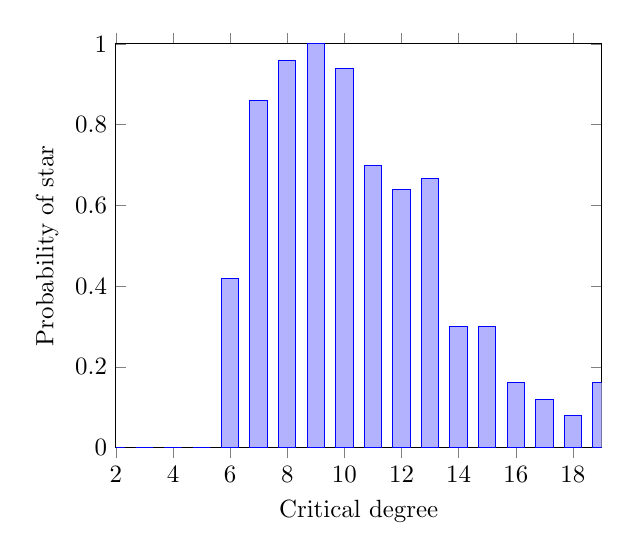
\begin{tikzpicture}[thick,scale=0.9]
\begin{axis}[
x tick label style={
	/pgf/number format/1000 sep=},
	ylabel=Probability of star,
	xlabel=Critical degree,
enlargelimits=0.0,
legend style={at={(0.5,-0.15)},
anchor=north,legend columns=-1},
ybar,
bar width=7pt,
]
\addplot
coordinates {
(2,0.0) (3,0.0) (4,0.0) (5,0.0) (6,0.42) (7,0.86) 
(8,0.96) (9,1.0) (10,0.94) (11,0.70) (12,0.64)
 (13,0.667) (14,0.3) (15,0.3) 
(16,0.16) (17,0.12) (18,0.08) (19,0.16) };
\end{axis}
\end{tikzpicture}
\caption{\label{fig:PlotStar} Shows the probability of the network ending up in a star, given different critical degrees.}
\end{figure}

From Figure \ref{fig:PlotClique} we can observe that the opposite is happening when the critical degree is increased; the probability of the resulting network being a clique drastically decreases. As we can see with a critical degree of seven or higher, it is very unlikely that we end up with a clique. These findings support our conjectures.

\begin{figure}
\centering
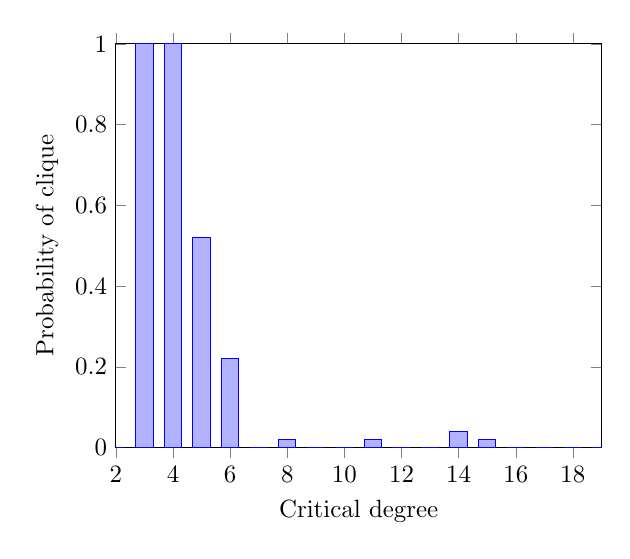
\begin{tikzpicture}[thick,scale=0.9]
\begin{axis}[
x tick label style={
	/pgf/number format/1000 sep=},
	ylabel=Probability of clique,
	xlabel=Critical degree,
enlargelimits=0.0,
legend style={at={(0.5,-0.15)},
anchor=north,legend columns=-1},
ybar,
bar width=7pt,
]
\addplot
coordinates {
(2,0.0)(3,1.0) (4,1.0) (5,0.52) (6,0.22) (7,0.0) 
(8,0.02) (9,0.0) (10,0.00) (11,0.02) (12,0.0)
 (13,0.0) (14,0.04) (15,0.02) 
(16,0.0) (17,0.0) (18,0.00) (19,0.0) };
\end{axis}
\end{tikzpicture}
\caption{\label{fig:PlotClique} Shows the probability of the network ending up in a clique, given different critical degrees.}
\end{figure}

In Figure \ref{fig:PlotStar} when the critical degree gets closer to the number of nodes in the network, the probability of the network evolving into a star decreases. However, in Figure \ref{fig:PlotStarIsj}, we have plotted the probability of the network evolving into a network where only a few(2-4) nodes end up with a high degree, but not necessarily a critical degree. As we see, this occurs with high probability from critical degree six and up. These networks are so called scale-free networks (A-B graphs, described in the methodology chapter), because there are a few hubs, that account for most of the connectivity in the network. The reason why we end up with a scale-free network is because nodes prefer to be connected with nodes with high connectivity, and thus will delete links to nodes with low connectivity. This is very similar to the simple model that creates scale-free networks, where the probability of connecting to a node is proportional to the degree of the node.


\begin{figure}
\centering
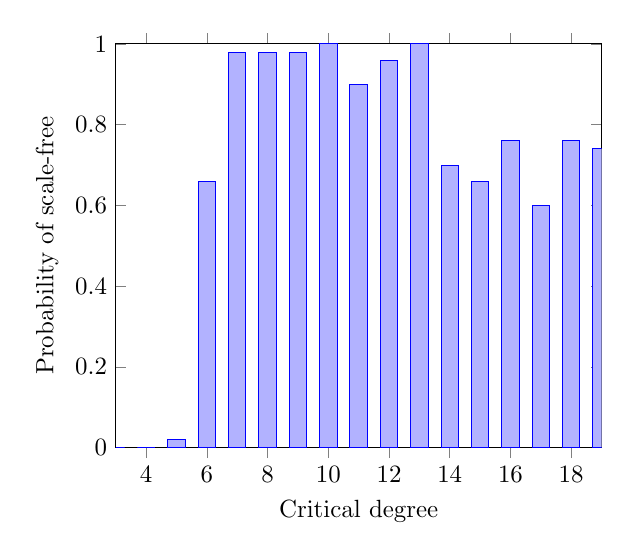
\begin{tikzpicture}[thick,scale=0.9]
\begin{axis}[
x tick label style={
	/pgf/number format/1000 sep=},
	ylabel=Probability of scale-free,
	xlabel=Critical degree,
enlargelimits=0.0,
legend style={at={(0.5,-0.15)},
anchor=north,legend columns=-1},
ybar,
bar width=7pt,
]
\addplot
coordinates {
(3,0.0) (4,0.0) (5,0.02) (6,0.66) (7,0.98) 
(8,0.98) (9,0.98) (10,1.00) (11,0.90) (12,0.96)
 (13,1) (14,0.7) (15,0.66) 
(16,0.76) (17,0.60) (18,0.76) (19,0.74) };
\end{axis}
\end{tikzpicture}
\caption{\label{fig:PlotStarIsj} Shows the probability of the network ending up in a scale-free structure, given different critical degrees.}
\end{figure}
\paragraph{Price of Anarchy.}
Another interesting thing is the average price of anarchy as function of the critical degree. The price of anarchy was calculated by taking the average total payoffs and dividing on the optimal payoff. The result can be seen in Figure \ref{fig:plotpriceofanarchy}. 

We see that the price of anarchy for the first critical degrees is 1, and then decreases until degree six, and at seven it increases again. This is because at degree one to five, the socially optimal structure is a clique. At degree six, a clique and a star, are almost equally good, and at degree seven and up, a star structure is the socially optimal outcome. 
In other words, when the cost is low, a clique is the optimal structure, and when the cost is high a star is the optimal structure. 

This further improves our findings, because we have now shown how an insurer can determine the resulting network formation by changing the cost. In addition, the formation that evolves has a price of anarchy close to 1. 

\begin{figure}
\centering
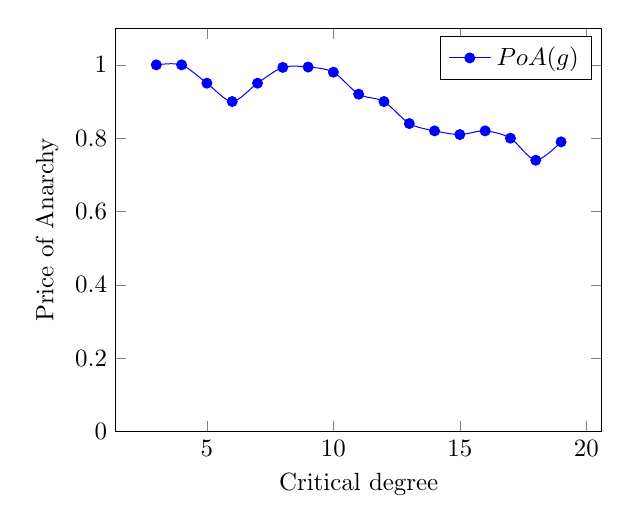
\begin{tikzpicture}[thick,scale=0.9]
\begin{axis}[
	ylabel=Price of Anarchy,
	ymin=0.0,
	xlabel=Critical degree]
\addplot [smooth,mark=*,blue] plot coordinates {

(3,1) (4,1) (5,0.95) (6,0.9) (7,0.95) 
(8,0.993) (9,0.994) (10,0.98) (11,0.92) (12,0.90)
 (13,0.84) (14,0.82) (15,0.81) 
(16,0.82) (17,0.8) (18,0.74) (19,0.79) };
\addlegendentry{$PoA(g)$}
\end{axis}
\end{tikzpicture}
\caption{\label{fig:plotpriceofanarchy} Shows the price of anarchy as a function of critical degree}
\end{figure}





\subsubsection{The General Case: Nontriviality.}
%
We assume that $H$ is
$\left(A_{\infty}, B_{\infty}\right)$-subqua\-dra\-tic at
infinity, for some constant \dots
%
\paragraph{Notes and Comments.}
The first results on subharmonics were \dots
%
\begin{proposition}
Assume $H'(0)=0$ and $ H(0)=0$. Set \dots
\end{proposition}
\begin{proof}[of proposition]
Condition (8) means that, for every $\delta'>\delta$, there is
some $\varepsilon>0$ such that \dots \qed
\end{proof}
%
\begin{example}[{{\rmfamily External forcing}}]
Consider the system \dots
\end{example}
\begin{corollary}
Assume $H$ is $C^{2}$ and
$\left(a_{\infty}, b_{\infty}\right)$-subquadratic
at infinity. Let \dots
\end{corollary}
\begin{lemma}
Assume that $H$ is $C^{2}$ on $\bbbr^{2n}\backslash \{0\}$
and that $H''(x)$ is \dots
\end{lemma}
\begin{theorem}[Ghoussoub-Preiss]
Let $X$ be a Banach Space and $\Phi:X\to\bbbr$ \dots
\end{theorem}
\begin{definition}
We shall say that a $C^{1}$ function $\Phi:X\to\bbbr$ satisfies \dots
\end{definition}
%
\section{Fine Tuning of the Text}
%
The following should be used to improve the readability of the text:
\begin{flushleft}
\begin{tabular}{@{}p{.19\textwidth}p{.79\textwidth}}
\verb|\,|   & a thin space, e.g.\ between numbers or between units
              and num\-bers; a line division will not be made
              following this space\\
\verb|--|   & en dash; two strokes, without a space at either end\\
\verb*| -- |& en dash; two strokes, with  a space at either end\\
\verb|-|    & hyphen; one stroke, no space at either end\\
\verb|$-$|  & minus, in the text {\em only} \\[8mm]
{\em Input} & \verb|21\,$^{\circ}$C etc.,|\\
            &  \verb|Dr h.\,c.\,Rockefellar-Smith \dots|\\
            & \verb|20,000\,km and  Prof.\,Dr Mallory \dots|\\
            & \verb|1950--1985 \dots|\\
            & \verb|this -- written on a computer -- is now printed|\\
            & \verb|$-30$\,K \dots|\\[3mm]
{\em Output}& 21\,$^{\circ}$C etc., Dr h.\,c.\,Rockefellar-Smith \dots\\
            & 20,000\,km and  Prof.\,Dr Mallory \dots\\
            & 1950--1985 \dots\\
            & this -- written on a computer -- is now printed\\
            & $-30$\,K \dots
\end{tabular}
\end{flushleft}
%
\section {Special Typefaces}
%
Normal type (roman text) need not be coded. {\itshape Italic}
(\verb|{\em <text>}| better still \verb|\emph{<text>}|) or, if
necessary, {\bfseries boldface} should be used for emphasis.\\[6pt]
\begin{minipage}[t]{\textwidth}
\begin{flushleft}
\begin{tabular}{@{}p{.25\textwidth}@{\hskip6pt}p{.73\textwidth}@{}}
\verb|{\itshape Text}|   & {\itshape Italicized Text}\\[2pt]
\verb|{\em Text}|   & {\em Emphasized Text --
   if you would like to emphasize a {\em definition} within an
   italicized text (e.g.\ of a {\em theorem)} you should code the
   expression to be emphasized by} \verb|\em|.\\[2pt]
\verb|{\bfseries Text}|& {\bfseries Important Text}\\[2pt]
\verb|\vec{Symbol}| & Vectors may only appear in math mode. The default
   \LaTeX{} vector symbol has been adapted\footnotemark\
 to LLNCS conventions.\\[2pt]
 & \verb|$\vec{A \times B\cdot C}| yields $\vec{A\times B\cdot C}$\\
 & \verb|$\vec{A}^{T} \otimes \vec{B} \otimes|\\
 & \verb|\vec{\hat{D}}$|yields $\vec{A}^{T} \otimes \vec{B} \otimes
\vec{\hat{D}}$
\end{tabular}
\end{flushleft}
\end{minipage}

\footnotetext{If you absolutely must revive the original \LaTeX{}
design of the vector symbol (as an arrow accent), please specify the
option \texttt{[orivec]} in the \texttt{documentclass} line.}
\newpage
%
\section {Footnotes}
%
Footnotes within the text should be coded:
\begin{verbatim}
\footnote{Text}
\end{verbatim}
{\itshape Sample Input}
\begin{flushleft}
Text with a footnote\verb|\footnote{The |{\tt footnote is automatically
numbered.}\verb|}| and text continues \dots
\end{flushleft}
{\itshape Sample Output}
\begin{flushleft}
Text with a footnote\footnote{The footnote is automatically numbered.}
and text continues \dots
\end{flushleft}
%
\section {Lists}
%
Please code lists as described below:\\[2mm]
{\itshape Sample  Input}
\begin{verbatim}
\begin{enumerate}
  \item First item
  \item Second item
  \begin{enumerate}
    \item First nested item
    \item Second nested item
  \end{enumerate}
  \item Third item
\end{enumerate}
\end{verbatim}
{\itshape Sample Output}
 \begin{enumerate}
\item First item
\item Second item
  \begin{enumerate}
    \item First nested item
    \item Second nested item
  \end{enumerate}
\item Third item
\end{enumerate}
%
\section {Figures}
%
Figure environments should be inserted after (not in)
the  paragraph in which the figure is first mentioned.
They will be numbered automatically.

Preferably the images should be enclosed as PostScript files -- best as
EPS data using the epsfig package.

If you cannot include them into your output this way and use other
techniques for a separate production,
the figures (line drawings and those containing halftone inserts
as well as halftone figures) {\em should not be pasted into your
laserprinter output}. They should be enclosed separately in camera-ready
form (original artwork, glossy prints, photographs and/or slides). The
lettering should be suitable for reproduction, and after a
probably necessary reduction the height of capital letters should be at
least 1.8\,mm and not more than 2.5\,mm.
Check that lines and other details are uniformly black and
that the lettering on figures is clearly legible.

To leave the desired amount of space for the height of
your figures, please use the coding described below.
As can be seen in the output, we will automatically
provide 1\,cm space above and below the figure,
so that you should only leave the space equivalent to the size of the
figure itself. Please note that ``\verb|x|'' in the following
coding stands for the actual height of the figure:
\begin{verbatim}
\begin{figure}
\vspace{x cm}
\caption[ ]{...text of caption...}          (Do type [ ])
\end{figure}
\end{verbatim}
\begin{flushleft}
{\itshape Sample Input}
\end{flushleft}
\begin{verbatim}
\begin{figure}
\vspace{2.5cm}
\caption{This is the caption of the figure displaying a white
eagle and a white horse on a snow field}
\end{figure}
\end{verbatim}
\begin{flushleft}
{\itshape Sample Output}
\end{flushleft}
\begin{figure}
\vspace{2.5cm}
\caption{This is the caption of the figure displaying a white eagle and
a white horse on a snow field}
\end{figure}
%
\section{Tables}
%
Table captions should be treated
in the same way as figure legends, except that
the table captions appear {\itshape above} the tables. The tables
will be numbered automatically.
%
\subsection{Tables Coded with \protect\LaTeX{}}
%
Please use the following coding:\\[2mm]
{\itshape Sample Input}
\begin{verbatim}
\begin{table}
\caption{Critical $N$ values}
\begin{tabular}{llllll}
\hline\noalign{\smallskip}
${\mathrm M}_\odot$ & $\beta_{0}$ & $T_{\mathrm c6}$ & $\gamma$
  & $N_{\mathrm{crit}}^{\mathrm L}$
  & $N_{\mathrm{crit}}^{\mathrm{Te}}$\\
\noalign{\smallskip}
\hline
\noalign{\smallskip}
 30 & 0.82 & 38.4 & 35.7 & 154 & 320 \\
 60 & 0.67 & 42.1 & 34.7 & 138 & 340 \\
120 & 0.52 & 45.1 & 34.0 & 124 & 370 \\
\hline
\end{tabular}
\end{table}
\end{verbatim}

\medskip\noindent{\itshape Sample Output}
\begin{table}
\caption{Critical $N$ values}
\begin{center}
\renewcommand{\arraystretch}{1.4}
\setlength\tabcolsep{3pt}
\begin{tabular}{llllll}
\hline\noalign{\smallskip}
${\mathrm M}_\odot$ & $\beta_{0}$ & $T_{\mathrm c6}$ & $\gamma$
  & $N_{\mathrm{crit}}^{\mathrm L}$
  & $N_{\mathrm{crit}}^{\mathrm{Te}}$\\
\noalign{\smallskip}
\hline
\noalign{\smallskip}
 30 & 0.82 & 38.4 & 35.7 & 154 & 320 \\
 60 & 0.67 & 42.1 & 34.7 & 138 & 340 \\
120 & 0.52 & 45.1 & 34.0 & 124 & 370 \\
\hline
\end{tabular}
\end{center}
\end{table}

Before continuing your text you need an empty line. \dots

\vspace{3mm}
For further information you will find a complete description of
the tabular environment
on p.~62~ff. and p.~204 of the {\em \LaTeX{} User's Guide \& Reference
Manual\/} by Leslie Lamport.
%
\subsection{Tables Not Coded with \protect\LaTeX{}}
%
If you do not wish to code your table using \LaTeX{}
but prefer to have it reproduced separately,
proceed as for figures and use the following coding:\\[2mm]
{\itshape Sample Input}
\begin{verbatim}
\begin{table}
\caption{text of your caption}
\vspace{x cm}     % the actual height needed for your table
\end{table}
\end{verbatim}
%
\subsection{Signs and Characters}
%
\subsubsection*{Special Signs.}
%
You may need to use special signs.  The available ones are listed in the
{\em \LaTeX{} User's Guide \& Reference Manual\/} by Leslie Lamport,
pp.~41\,ff.
We have created further symbols for math mode (enclosed in \$):
\begin{center}
\begin{tabular}{l@{\hspace{1em}yields\hspace{1em}}
c@{\hspace{3em}}l@{\hspace{1em}yields\hspace{1em}}c}
\verb|\grole| & $\grole$ & \verb|\getsto| & $\getsto$\\
\verb|\lid|   & $\lid$   & \verb|\gid|    & $\gid$
\end{tabular}
\end{center}
%
\subsubsection*{Gothic (Fraktur).}
%
If gothic letters are {\itshape necessary}, please use those of the
relevant \AmSTeX{} alphabet which are available using the amstex
package of the American Mathematical Society.

In \LaTeX{} only the following gothic letters are available:
\verb|$\Re$| yields $\Re$ and \verb|$\Im$| yields $\Im$. These should
{\itshape not\/} be used when you need gothic letters for your contribution.
Use \AmSTeX{} gothic as explained above. For the real and the imaginary
parts of a complex number within math mode you should use instead:
\verb|$\mathrm{Re}$| (which yields Re) or \verb|$\mathrm{Im}$| (which
yields Im).
%
\subsubsection*{Script.}
%
For script capitals use the coding
\begin{center}
\begin{tabular}{l@{\hspace{1em}which yields\hspace{1em}}c}
\verb|$\mathcal{AB}$| & $\mathcal{AB}$
\end{tabular}
\end{center}
(see p.~42 of  the \LaTeX{} book).
%
\subsubsection*{Special Roman.}
%
If you need other symbols than those below, you could use
the blackboard bold characters of \AmSTeX{},  but there might arise
capacity problems
in loading additional \AmSTeX{} fonts. Therefore  we created
the blackboard bold characters listed below.
Some of them are not esthetically
satisfactory. This need not deter you from using them:
in the final printed form they will be
replaced by the well-designed MT (monotype) characters of
the phototypesetting machine.
\begin{flushleft}
\begin{tabular}{@{}ll@{ yields }
c@{\hspace{1.em}}ll@{ yields }c}
\verb|\bbbc| & (complex numbers)   & $\bbbc$
  & \verb|\bbbf| & (blackboard bold F) & $\bbbf$\\
\verb|\bbbh| & (blackboard bold H) & $\bbbh$
  & \verb|\bbbk| & (blackboard bold K) & $\bbbk$\\
\verb|\bbbm| & (blackboard bold M) & $\bbbm$
  & \verb|\bbbn| & (natural numbers N) & $\bbbn$\\
\verb|\bbbp| & (blackboard bold P) & $\bbbp$
  & \verb|\bbbq| & (rational numbers)  & $\bbbq$\\
\verb|\bbbr| & (real numbers)      & $\bbbr$
  & \verb|\bbbs| & (blackboard bold S) & $\bbbs$\\
\verb|\bbbt| & (blackboard bold T) & $\bbbt$
  & \verb|\bbbz| & (whole numbers)     & $\bbbz$\\
\verb|\bbbone| & (symbol one)      & $\bbbone$
\end{tabular}
\end{flushleft}
\begin{displaymath}
\begin{array}{c}
\bbbc^{\bbbc^{\bbbc}} \otimes
\bbbf_{\bbbf_{\bbbf}} \otimes
\bbbh_{\bbbh_{\bbbh}} \otimes
\bbbk_{\bbbk_{\bbbk}} \otimes
\bbbm^{\bbbm^{\bbbm}} \otimes
\bbbn_{\bbbn_{\bbbn}} \otimes
\bbbp^{\bbbp^{\bbbp}}\\[2mm]
\otimes
\bbbq_{\bbbq_{\bbbq}} \otimes
\bbbr^{\bbbr^{\bbbr}} \otimes
\bbbs^{\bbbs_{\bbbs}} \otimes
\bbbt^{\bbbt^{\bbbt}} \otimes
\bbbz \otimes
\bbbone^{\bbbone_{\bbbone}}
\end{array}
\end{displaymath}
%
\section{References}
\label{refer}
%
There are three reference systems available; only one, of course,
should be used for your contribution. With each system (by
number only, by letter-number or by author-year) a reference list
containing all citations in the
text, should be included at the end of your contribution placing the
\LaTeX{} environment \verb|thebibliography| there.
For an overall information on that environment
see the {\em \LaTeX{} User's Guide \& Reference
Manual\/} by Leslie Lamport, p.~71.

There is a special {\sc Bib}\TeX{} style for LLNCS that works along
with the class: \verb|splncs.bst|
-- call for it with a line \verb|\bibliographystyle{splncs}|.
If you plan to use another {\sc Bib}\TeX{} style you are customed to,
please specify the option \verb|[oribibl]| in the
\verb|documentclass| line, like:
\begin{verbatim}
\documentclass[oribibl]{llncs}
\end{verbatim}
This will retain the original \LaTeX{} code for the bibliographic
environment and the \verb|\cite| mechanism that many {\sc Bib}\TeX{}
applications rely on.
%
\subsection{References by Letter-Number or by Number Only}
%
References are cited in the text -- using the \verb|\cite|
command of \LaTeX{} -- by number or by letter-number in square
brackets, e.g.\ [1] or [E1, S2], [P1], according to your use of the
\verb|\bibitem| command in the \verb|thebibliography| environment. The
coding is as follows: if you choose your own label for the sources by
giving an optional argument to the \verb|\bibitem| command the citations
in the text are marked with the label you supplied. Otherwise a simple
numbering is done, which is preferred.
\begin{verbatim}
The results in this section are a refined version
of \cite{clar:eke}; the minimality result of Proposition~14
was the first of its kind.
\end{verbatim}
The above input produces the citation: ``\dots\ refined version of
[CE1]; the min\-i\-mality\dots''. Then the \verb|\bibitem| entry of
the \verb|thebibliography| environment should read:
\begin{verbatim}
\begin{thebibliography}{[MT1]}
.
.
\bibitem[CE1]{clar:eke}
Clarke, F., Ekeland, I.:
Nonlinear oscillations and boundary-value problems for
Hamiltonian systems.
Arch. Rat. Mech. Anal. {\bfseries 78} (1982) 315--333
.
.
\end{thebibliography}
\end{verbatim}
The complete bibliography looks like this:
%
\begin{thebibliography}{[MT1]}
%
\bibitem[CE1]{clar:eke}
Clarke, F., Ekeland, I.:
Nonlinear oscillations and
boundary-value problems for Hamiltonian systems.
Arch. Rat. Mech. Anal. {\bfseries 78} (1982) 315--333
%
\bibitem[CE2]{clar:eke:2}
Clarke, F., Ekeland, I.:
Solutions p\'{e}riodiques, du
p\'{e}riode donn\'{e}e, des \'{e}quations hamiltoniennes.
Note CRAS Paris {\bfseries 287} (1978) 1013--1015
%
\bibitem[MT1]{mich:tar}
Michalek, R., Tarantello, G.:
Subharmonic solutions with prescribed minimal
period for nonautonomous Hamiltonian systems.
J. Diff. Eq. {\bfseries 72} (1988) 28--55
%
\bibitem[Ta1]{tar}
Tarantello, G.:
Subharmonic solutions for Hamiltonian
systems via a $\bbbz_{p}$ pseudoindex theory.
Annali di Matematica Pura (to appear)
%
\bibitem[Ra1]{rab}
Rabinowitz, P.:
On subharmonic solutions of a Hamiltonian system.
Comm. Pure Appl. Math. {\bfseries 33} (1980) 609--633
\end{thebibliography}
%
\subsubsection*{Number-Only System.}
%
For this preferred system do not use the optional argument
in the \verb|\bibitem| command: then, only numbers will
appear for the citations in the text (enclosed in square brackets)
as well as for the marks in your
bibliography (here the number is only end-punctuated without
square brackets).

Subsequent citation numbers in the text are collapsed to ranges.
Non-numeric and undefined labels are handled correctly but no sorting is
done.

E.g., \verb|\cite{n1,n3,n2,n3,n4,n5,foo,n1,n2,n3,?,n4,n5}| -- where
\verb|n|$x$ is the key of the $x^{\mathrm{th}}$ \verb|\bibitem|
command in sequence, \verb|foo| is the key of a \verb|\bibitem| with an
optional argument, and \verb|?| is an undefined reference -- gives
1,3,2-5,foo,1-3,?,4,5 as the citation reference.

\begin{verbatim}
\begin{thebibliography}{1}
\bibitem {clar:eke}
Clarke, F., Ekeland, I.:
Nonlinear oscillations and boundary-value problems for
Hamiltonian systems.
Arch. Rat. Mech. Anal. {\bfseries 78} (1982) 315--333
\end{thebibliography}
\end{verbatim}
%
\subsection{Author-Year System}
%
References are cited in the text by name and year in parentheses
and should look as follows:
(Smith 1970, 1980), (Ekeland et al. 1985, Theorem 2), (Jones and Jaffe
1986; Farrow 1988, Chap.\,2). If the name is part of the sentence
only the year may appear in parentheses,
e.g.\ Ekeland et al. (1985, Sect.\,2.1)
The reference list should contain all citations occurring in the text,
ordered alphabetically by surname (with initials following). If there
are several works by the same author(s) the references should be listed
in the appropriate order indicated below:
\begin{alpherate}
\setlength{\hfuzz}{5pt}
\item
One author: list works chronologically;
\item
Author and same co-author(s): list works chronologically;
\item
Author and different co-authors: list works alphabetically
according to co-authors.
\end{alpherate}
If there are several works by the same author(s) and in the same year,
but which are cited separately, they should be distinguished by the use
of ``a'', ``b'' etc., e.g.\ (Smith 1982a), (Ekeland et al. 1982b).
%
\subsubsection*{How to Code Author-Year System.}
%
If you want to use this system you have to specify the option
\verb|[citeauthoryear]| in the \verb|documentclass|, like:
\begin{verbatim}
\documentclass[citeauthoryear]{llncs}
\end{verbatim}
Write your citations in the text explicitly except for the year, leaving
that up to \LaTeX{} with the \verb|\cite| command. Then give only the
appropriate year as the optional argument (i.e. the label in square
brackets) with the \verb|\bibitem| command(s).\\[2mm]
{\itshape Sample Input}
\begin{verbatim}
The results in this section are a refined version
of Clarke and Ekeland (\cite{clar:eke}); the minimality result of
Proposition~14 was the first of its kind.
\end{verbatim}
The above input produces the citation: ``\dots\ refined version of
Clarke and Ekeland (1982); the minimality\dots''. Then the
\verb|\bibitem| entry of \verb|clar:eke| in the \verb|thebibliography|
environment should read:
\begin{verbatim}
\begin{thebibliography}{}  % (do not forget {})
.
.
\bibitem[1982]{clar:eke}
Clarke, F., Ekeland, I.:
Nonlinear oscillations and boundary-value problems for
Hamiltonian systems.
Arch. Rat. Mech. Anal. {\bfseries 78} (1982) 315--333
.
.
\end{thebibliography}
\end{verbatim}
{\itshape Sample Output}
\bibauthoryear
%
\end{document}
